\documentclass[english]{article}
%\usepackage{sansseriftitles}
\usepackage{1inchmargins}
\usepackage[iso]{isodate}
\usepackage{hyperref}
\usepackage{color}
\usepackage{booktabs}
\usepackage{amsmath}
\usepackage{graphicx}
\renewcommand{\familydefault}{\sfdefault}
\renewcommand{\tabcolsep}{8pt}

\hypersetup{
    colorlinks=true,
    urlcolor=blue,
}

\newcommand{\surl}[1]{{\small \url{#1}}}

\begin{document}


\centerline{\sf \Huge AstroTortilla User Guide}
\centerline{Latest update: \today}

\tableofcontents

\setlength{\parindent}{0pt}
\setlength{\parskip}{2ex}


\newpage

\section{Introduction}

\emph{Blind plate solving} makes it possible to identify an astrophotograph's location in the sky without knowing anything else about it. \emph{AstroTortilla} utilizes blind plate solving to automatically tell your mount where your telescope is pointing at, making computer controlled astrophotography easier than ever -- with no cost.

AstroTortilla is a wrapper that makes the software you already use (computer control of your camera and GoTo tracking mount) talk to a plate solver application.

Even when doing a GoTo-slew over a very large distance on the sky, AstroTortilla centers your target within the arcsecond, in one or two iterations -- no matter how bad the GoTo-calibration.

Plate solver assisted GoTo also makes polar alignment a one minute job. Just let AstroTortilla look around and take a few images. The polar alignment error is calculated and shown in degrees. What's left for you is to turn the knobs.

\emph{Mexican tortillas} are commonly prepared with meat to make dishes such as
tacos, burritos, and enchiladas. \emph{AstroTortilla} wraps itself around a
bunch of useful software for a tasty nocturnal snack under the starry night
sky.


\section{Compatibility with other software and equipment} 

\subsection{Camera control}

For using AstroTortilla, you need a way to get the images from the camera to your computer. Currently the following ways to connect a camera are supported:
\begin{itemize}
\item \textbf{MaxIm DL} by Diffraction Limited
\item \textbf{Nebulosity 2 and 3} by Stark Labs
\item \textbf{Astro Photography Tool} by Incanus
\item \textbf{Screen capture} from any other software (like \emph{PHD Guiding} or \emph{BackyardEOS})
\item Direct connection via \textbf{ASCOM interface}
\item Manually \textbf{pointing to an image file} on your hard drive
\end{itemize}

We are looking forward to a native support of \emph{BackyardEOS} as well as other camera control software in the future. Users are encouraged to develop interfaces for support of more imaging software options, just drop us an email!

\subsection{GoTo mount control}

AstroTortilla currently supports any computerized tracking mount with an
\hbox{\textbf{{ASCOM interface}}}.  The field testing of AstroTortilla
functions under the night sky is carried out with EQMOD software controlling
Sky-Watcher HEQ5 and EQ6 mounts. Users have also reported successful usage of with Celestron CG-5 and Gemini G42 mounts as well as many other ASCOM-drived mounts.

Due to ASCOM, AstroTortilla is currently limited to a Windows platform. INDI + Linux might be possible some day.


\subsection{Plate solving}

Plate solving is the sport of identifying the shapes drawn by the locations of
stars in an astronomical image. Once the stars are identified, this astrometric
solution can be used to work out the coordinates of the center of the frame,
the width an height of the field of view, the rotational angle of the image
with respect to celestial coordinate axes, the angular resolution of one pixel
in the imaging setup and, by knowing the pixel size of the sensor, the exact
focal length of the imaging objective used.

Normally, a stellar catalog, that is, a database of star locations and a rough
estimate of where the telescope was pointed at during exposure are needed to
successfully plate solve an image.

\subsubsection{Astrometry.net}

The Astrometry.net project is a revolutionary effort of developing means of
working out the astrometric solution of any astronomical image with no initial
knowledge of the imaging parameters \emph{whatsoever}. The project will make
its engine, algorithms and code freely avaible to the public. The key to
blindfolded fast plate solving is doing most of the laborous calculation beforehand, 
by prebuilding \emph{huge} catalogs of cleverly sorted four-star patterns of the entire sky.

At the time of writing Astrometry.net is in beta testing phase. An online user
interface for plate solving your images is at
\surl{http://nova.astrometry.net}.  Astrometry.net can also be run locally in a
Linux, Unix, Mac box or Cygwin for Windows environment.

AstroTortilla uses the local version of Astrometry.net which runs in Cygwin. We've made everything as easy as possible -- the AstroTortilla installer program fetches everything you need online.

Some day, AstroTortilla might support solving images online for imaging setups with limited hard drive and CPU capacity, but a working internet connection. For now, however, it's not yet possible, due to the incomplete Astrometry.net online API.

\newpage

\section{Installing AstroTortilla}

The installation is easy since the AstroTortilla installer now includes everything you need. A Cygwin environment with a working build of Astrometry.net is automatically set up on your PC. The installer will download the index files (i.e. star catalogs) needed for plate solving, customized to match the field of view of your imaging gear.

Cygwin takes up some 300 MB of space on your hard drive. In addition to being essential to make AstroTortilla run Astrometry.net, Cygwin provides you a handy set of Linux-like command line tools which you might or might not need. If you don't, no sweat, for using AstroTortilla there's no need to touch the scary command line terminals.

The index files (databases) needed for plate solving however will use up even more
space. If you use camera optics or short refractors, about 1 GB of indices are needed.
Smaller fields (longer telescopes) require additional levels of index files. 
Every level doubles in size. All index files take up 25 GB of space.

The smallest field solvable with Astrometry.net is about five arc minutes. 

%\subsection*{\refstepcounter{subsection}\thesubsection\quad Getting the installer}
\subsection{Get the installer}

You'll find the installer at \surl{http://astrotortilla.sourceforge.net/}.
Download and run \\\texttt{AstroTortilla-<version>-x86.exe}. 

If you know what 64-bit means, try the x64 version.

%\subsection*{\refstepcounter{subsection}\thesubsection\quad Select Components}
\subsection{Select Components}

Once past the first steps of the installer, choose between the following options on what to install:
\begin{description}
\item [Install AstroTortilla, Cygwin, astrometry.net and indexes (Default)] \hfill \\
Normally you should choose this option which will install everything you need. 

\item [Install AstroTortilla, Cygwin and astrometry.net without indexes]\hfill \\
Use this option if you don't yet know your Field of View, or want to get the index files later for some other reason.

\item [Install AstroTortilla only] \hfill \\
This option can be used to update an old or uninstalled AstroTortilla and not touching a working Astrometry.net setup in Cygwin.

\item [Install Additional index files] \hfill \\
If you didn't download any index files the first time or upgraded to a longer focal length, fetch more files with this option.

\item [Update Cygwin, astrometry.net and install index files.] \hfill \\
When Astrometry.net is updated, we'll build you a new Cygwin version. Use this option to update.

\end{description}

Normally just select the first one!

{\scriptsize \textbf{Note to Cygwin users:} If you already have Cygwin installed for some other reason, we assume you know your way around it. There is an official \texttt{setup.exe} wrapped in the AstroTortilla installer. astrometry.net isn't provided on any official Cygwin repository, but the AstroTortilla installer uses our own custom mirror. In this case, choose to install everything and point the installer to your Cygwin directory.}

\subsection{Choose index files}

{\scriptsize \textbf{Impatient?} If you image below $f$=1000 mm, skip the math and just get levels 4004--4019! (ca. 2 GB)}

Next you need to specify which index files you want the installer to fetch. The correct options depend on the field of view (FOV) of your imaging gear. 

You can use an online FOV calculator or the this (approximate) formula:
\[
\text{FOV (\ensuremath{^\circ})}=\frac{57.3\times\text{Sensor size}}{\text{Focal length}}
\]
Choose the same units for both Sensor size and Focal length, e.g., 17 mm and 1200 mm. As Sensor size, choose any dimension (height, width, diagonal), exact values don't matter. For arc minutes, multiply the result by 60.

The plate solver will search through your image for \emph{quads} (four-star constellations) to recognize. The quads will be from 10\% to 100\% the size of your image. Choose a level or a few that contain quads of matching size.

\textbf{Example:} With the values 17 mm and 1200 mm as above, $\text{FOV} \approx 0.8^\circ \approx 50'$. Levels 4004 trough 4009 span quads of $8' \text{ to } 60'$. A few more MB doesn't matter, so let's choose everything from 4004 to 4019! Those will take up about 2~GB of space total.

\begin{table}[!h]
\centering
\begin{tabular}{r r r @{ } c @{ } l r @{ } c @{ } l} \toprule
Index level 	& Size (MB) & \multicolumn{3}{r}{Quads ($^\circ$)} & \multicolumn{3}{r}{Quads (')} \\ \midrule
4000 & 11 GB 	&  	&--& 		& 2 	&--&	2.8\\
4001 & 7 GB 	&  	&--&  	& 2.8	&--&	4\\
4002 & 4 GB 	&  	&--&  	& 4 	&--&	5.6\\
4003 & 2	GB 	&  	&--&  	& 5.6	&--&	8\\
4004 & 960  	&  	&--&  	& 8 	&--&	11\\
4005 & 470  	&  	&--&  	& 11 	&--&	16\\
4006 & 230  	&  	&--&  	& 16 	&--&	22\\
4007 & 115  	&    	&--&  	& 22 	&--&	30\\
4008 & 62  		& 0.5 &--& 0.7	& 30 	&--&	42\\
4009 & 31  		& 0.7 &--& 1	& 42 	&--&	60\\
4010 & 15  		& 1 	&--& 1.4	& 60 	&--&	85\\
4011 & 5.6  	& 1.4	&--& 2	& 85 	&--&	120\\
4012 & 2.8  	& 2 	&--& 2.8	& 120 &--&	170\\
4013 & 1.4  	& 2.8	&--& 4 	& 170	&--&	240\\
4014 & 0.7  	& 4	&--& 5.6	&		&--&		\\
4015 & 0.4  	& 5.6	&--& 8 	&		&--&		\\
4016 & 0.2  	& 8	&--& 11	&		&--&		\\
4017 & 0.09  	& 11	&--& 17	&		&--&		\\
4018 & 0.06  	& 17	&--& 23	&		&--&		\\
4019 & 0.04  	& 23	&--& 33	&		&--&		\\ \bottomrule
\end{tabular}
\end{table}

Should you ever run this step again to fetch new index levels, you can leave the widest index as 4019. AstroTortilla is aware of which index files you already have and only downloads the additional ones you want.

\subsection{Finalize installation}

Next, just click through the rest of the installation. Now you'll be able to launch AstroTortilla to test-solve some old frames. Maybe use an ASCOM simulator for the scope, connected to a planetarium software to virtually slew to the locations of your solved images.

\newpage

\section{AstroTortilla usage}

\subsection{Main screen}

The main screen consists of four panels: Telescope, Camera, Solver and Actions.

\begin{figure}[h!]
\centering
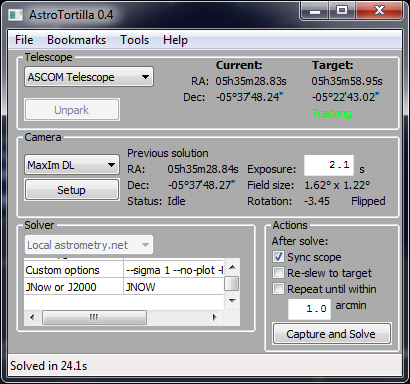
\includegraphics[width=0.6\textwidth]{Tortilla-v04-screen-en.png}
\end{figure}

%\textbf{\emph{Telescope panel}} 
\subsubsection{Telescope panel}

In the drop-down menu, select \textbf{ASCOM Telescope} and then choose the Correct 
ASCOM driver for your telescope/mount. You can also choose a simulator.

For useful operation, the ASCOM driver of your mount should work as a hub.
This is the normal operation of, for instance, EQMOD and Astro-Physics
ASCOM-drivers. If your driver only supports one software connection at a 
time, check out Plain Old Telescope Handset (POTH).

\subsubsection{Camera panel}

Select a way to connect to your camera. There's native support for \textbf{Astro Photography Tool}, \textbf{MaxIm DL} and \textbf{Nebulosity 2/3}. 

With MaxIm DL and Nebulosity you can set the imaging filter and binning used for AstroTortilla-related exposures. With Nebulosity you should also set the image directory reset, as we currently cannot read the value from Nebulosity. AstroTortilla provides two macros for giving the current date, \textit{\%(date)s} for current date and \textit{\%(night)s} for rolling the date at noon. Both are formatted as YYYY-MM-DD. There is typically no need to select the actual camera for Nebulosity.

If you use other software, try \textbf{Screen Capture}. Working settings for PHD Guiding are provided. For other software configure the capture area yourself.

For manual operation or indoors tests, choose \textbf{File Open dialog}. AstroTortilla then asks you for a file every time it needs to "Capture" an image.

You can also directly connect to an \textbf{ASCOM Camera}.

AstroTortilla cannot reliably auto-start your imaging application, it is recommended that you take one exposure in the imaging application itself to verify equipment functionality and focus.

\subsubsection{Solver panel}

In the solver panel, \textbf{Local astrometry.net} is the only option for now. You can tweak solver settings in the table below.

\subsubsection{Actions panel}

Here, choose what to do after successfully capturing and solving an image.
\begin{description}
\item[Sync scope] \hfill \\
Tell the scope it's pointing at the coordinates of the solution.
\item[Re-slew to target] \hfill \\
Correct the pointing of the scope to where the GoTo \emph{thought} it was pointing earlier.
\item[Repeat until within ... arcmin] \hfill \\
Iterate the above two until the scope points exactly at the target, within the tolerance specified.
\end{description}

\subsection{Normal workflow}

After connecting to your equipment and software, slew to a target with your telescope control software or planetarium application.
Now \emph{Target} shows the coordinates of the object you selected, and \emph{Current} shows the same coordinates since this is
where the mount thinks it pointing at at this stage. Those might, however, be more or less incorrect.

Select some actions in the Actions panel (all three of them if you like) and a suitable 
exposure time in the Camera panel. Hit \emph{Capture and Solve}.

AstroTortilla now uses the camera to expose a frame and delivers it to the solver engine. 
After a successful plate solution, AstroTortilla becomes aware of the \emph{true} 
pointing direction of the scope and indicates the coordinates in the Camera panel.

If the \emph{Sync Scope} option was checked, the true coordinates are indicated
in "Current" at the Telescope panel, too, and the GoTo of your telescope is now
properly calibrated.

If the \emph{Re-slew to target} option was checked, AstroTortilla applies a new
slew command to the mount, to the coordinates your mount assumed it was
pointing at earlier. Usually your object will now be very close to the center
of your frame.

If \emph{Repeat until..} was checked, a new frame is exposed and used to refine the pointing 
even further. After two or three rounds your target should be exactly at the crosshair.
Be sure not to input a threshold value too low (i.e., lower than the mechanical pointing accuracy of your mount),
else AstroTortilla will repeat the process until the iteration limit (default of five iterations) is reached.

\subsection{Tools menu}
\subsubsection{Goto image tool}

The Goto image tool solves an image from your hard drive and slews the
telescope to its central coordinates. You can use it to return to the exact
framing of a previous night's exposing session, or mimic the framing of your
favourite Hubble Space Telescope shot, for example.

To use it, select \emph{Tools $\rightarrow$ Goto image} and select the image to
solve in the appearing dialog.  AstroTortilla then solves it and slew the
telescope to the coordinates of its center. The image has to be in FITS, JPEG,
TIFF or PNM format.

When using the Goto image tool, AstroTortilla ignores any check marks you've
entered in the Actions panel and always does iterative centering with the
threshold you entered in the bottom of the panel. The search radius parameter in
your Solver panel is also ignored - the Goto image is always a blind solve with a radius of 180$^\circ$.

\subsubsection{Polar Alignment}

Using a plate solver eliminates the waiting that's distinctive in polar aligning 
your mount with the traditional drift method. Just solve a frame, turn the scope 
along RA and solve again. The difference in solved declination values is equal 
to the amount of drift in declination observed when tracking a star for a time 
equal to the amount turned. A tedious 20 minute drift can now be done in way less than a minute!

A pair of frames shot at the east/west meridian is used to determine the
altitude error of the polar axis, and a pair shot at the southern meridian
(assuming northern hemisphere observation) gets you the azimuthal error.

To use the tool, select \emph{Tools $\rightarrow$ Polar Alignment}. Choose the
correct hemisphere and point your mount roughly at the meridian to measure
azimuth error or to the east or west to measure altitude error.

Then press the according button to let AstroTortilla shoot and solve the pair
of frames. When done, your polar alignment error in degrees is shown on the
screen. Use this to correct your alignment by turning the alignment knobs on
your mount.

When measuring azimuthal error, be sure not to point within a half a degree or
closer to the meridian to avoid meridian flips! Pointing on the west (right)
side of the southern meridian is the safest bet.

{\footnotesize \textbf{Note:} With clever choosing of pointing direction and some
spherical geometry, the polar alignment error on both axes can be calculated from 
just two frames! We hope to include this feature in a future version of AstroTortilla.}

\subsubsection{Drift shot tool}

For your convenience a non plate solver based polar alignment helper is also available.
If you want to spend your clear nights drift aligning, AstroTortilla makes it 
easier to observe the amount and direction of drift by
employing a technique introduced by Robert Vice in the September 2005 issue of
AstroPhoto Insight magazine. It involves slewing the mount eastward for a
specified amount of time, after which an equally long westward slew is done.

If there's any declination drift present, the star will trace a horizontal V
pattern. The image is exposed for a few seconds before starting the slews in
order to create a small blob to the other arm of the V to distinguish the
direction of drift.

When the alignment is correct, the V will converge into just a horizontal line.
For more information about the V-drift method, see
\surl{http://www.astrophotoinsight.com/node/568}.

To use the tool, point your telescope at a reasonably bright star and select
\emph{Tools $\rightarrow$ Drift shot}.  AstroTortilla then starts a exposing 
a frame and moves the mount back and forth. You can choose an exposure time of 
your choice in the Camera panel. The Drift shot exposure will, however, always 
be at least 30 seconds, even if a lower value is entered.

After the exposure is done, you can examine the resulting image in your camera 
control software to determine if your alignment causes any declination drift.

\subsection{Bookmarks}

In the Bookmarks menu, you can save plate solutions and accurately slew back to their location later. 
This is especially useful for multiple night exposure projects of targets that are framed off-center for whatever reason.

You can add bookmarks from the current solution after pointing the scope somewhere or from an image pointed from the hard drive. Or why not make a bookmark of the framing of your favorite APOD!

\subsection{Configuring AstroTortilla}

AstroTortilla can be configured various ways by editing the config file. You can also store multiple config files for quickly switching between
settings for various setups.

The plate solving process can be speeded up considerably by tweaking the solve-field command line parameters, most notably the \texttt{--sigma} option.

For detailed description of the various configuration options, refer to the AstroTortilla wiki entry on Configuration at
\surl{https://sourceforge.net/p/astrotortilla/home/Configuration/}

\section{Credits}

AstroTortilla is brought to you by Antti Kuntsi (Mickut), Lauri Kangas (Vostok), Samuli Vuorinen (naavis) and Jussi Kantola (ketarax). 

Special thanks to Ivaylo Stoynov for incorporating AstroTortilla remote connection support into APT.

%\begin{tabular}{l l}
%Antti Kuntsi (Mickut) &Main software development \\
%Lauri Kangas (Vostok) &Maxim DL plugin, documentation \\
%Samuli Vuorinen (naavis) &Polar alignment tool, Astrometry.net online plugin \\
%Jussi Kantola (ketarax) &Packaging Astrometry.net for easy installing \\
%\end{tabular}



\end{document}
